\documentclass[a4paper,12pt]{article}

\usepackage{cmap}					% поиск в PDF
\usepackage[T2A]{fontenc}			% кодировка
\usepackage[utf8]{inputenc}			% кодировка исходного текста
\usepackage[english,russian]{babel}	% локализация и переносы
\usepackage{enumitem}  				% смена типа символя у enumerate
\usepackage{amsmath,amsfonts,amssymb,amsthm,epsfig,epstopdf,titling,url,array}
\usepackage{icomma} 				% "Умная" запятая: $0,2$ --- число, $0, 2$ --- перечисление
\usepackage{hyperref}				% кликабельные ссылки
\usepackage{soulutf8} 				% Модификаторы начертания
\usepackage{mathtools}
\DeclarePairedDelimiter{\ceil}{\lceil}{\rceil}


\usepackage{multicol, caption}
\usepackage{lipsum}
\newenvironment{Figure}
	{\par\medskip\noindent\minipage{\linewidth}}
	{\endminipage\par\medskip}

\graphicspath { {img} }

\usepackage[ruled,
linesnumbered,
vlined]
{algorithm2e}				% красивые алгоритмы

\sloppy

\SetAlgorithmName{Алгоритм}{algo}{Список алгоритмов}
\SetKwInput{KwData}{Вход}
\SetKwInput{KwResult}{Выход}
\SetNlSty{textbf}{}{.}
\SetAlgoNlRelativeSize{0}
\SetKwIF{If}{ElseIf}{Else}{Если}{то}{иначе если}{иначе}{}
\SetKwFor{ForEach}{Для каждого}{}{fintq}%
\SetKwFor{While}{Пока}{}{fintq}%

\theoremstyle{definition}
\newtheorem{property}{Свойство}[subsection]
\renewcommand\theproperty{\arabic{property}}

\title{Контрольная работа \linebreak Вариант №4.}
\author{Роман Астраханцев, СКБ-171}

\begin{document}
	\maketitle
	
	\section*{Задача 1}
	Дана сеть Фейстеля, состоящая из 8 итераций, с длиной блока $n=128$ бит.
	Из мастер ключа $K=(K_1, K_2, K_3, K_4)$, где $K_1, \dots, K_4 \in V_{64}$, итерационные ключи (на итерациях $1, 2, 3, \dots, 8$) получаются вырабаютываются как последовательность $K_3, K_2, K_4, K_1, K_3, K_2, K_4, K_1$. Обозначим за $E: V_{128} \times V_{256} \rightarrow V_{128}$ алгоритм зашифрования.
	
	Описать трудоемкость, вероятность успеха, затраты по памяти и объём материала для методов тотального опробования и слайд-атаки.
		
		
	\begin{multicols}{2}
        \begin{Figure}
			\centering
			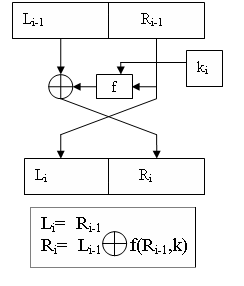
\includegraphics[width=\linewidth]{round.png}
			\captionof{figure}{Раунд сети Фейстеля}
		\end{Figure}

        \begin{Figure}
			\centering
			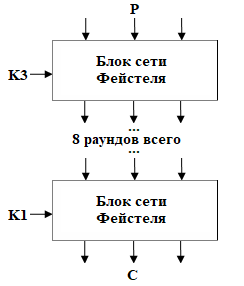
\includegraphics[width=\linewidth]{cpiher.png}
			\captionof{figure}{Шифр из задачи}
		\end{Figure}			
	\end{multicols}

	\subsection*{Метод тотального опробования}
	
	Для начала определим количество материала, необходимое для однозначного опредления ключа. Поскольку одной на паре $(P, C)$ открытого и шифрованного текста, где $P, C \in V_{128}$, можно отбраковать $2^{128}$ ключей, то потребуется $\ceil{\frac{256}{128}} = 2$ различные пары: $(P_1, C_1), (P_2, C_2)$. Будем дальше считать, что они нам даны.
	
	
	\begin{algorithm}[H]
		
		\caption{Метод тотального опробования}
		\label{alg:Total}
		\SetAlgoNoEnd
		
		\KwData{Пары открытого и шифрованного текста $(P_1, C_1), (P_2, C_2)$}
		\KwResult{Ключ шифрования $K$}
		
		\ForEach{$\tilde{k} \in V_{256}$}{ 
			Вычислить $B_1 = E(P_1, \tilde{k})$ \\
			\If{$B_1=C_1$,}{
				Вычислить $B_2 = E(P_2, \tilde{k})$ \\
				\If{$B_2=C_2$,}{
					Закончить алгоритм и вернуть $\tilde{k}$
				}
			}
		}
	\end{algorithm}	
	
	Трудоёмоксть $Q$ этого алгоритма будем измерять в количествах зашифрования, а необходимую для работы алгоритма память $M$ в битах. Тогда имеем
	
	\[ Q = 2^{256} + 2^{128} + 1 \approx 2^{256} \]
	
	\[ M = \alpha, \]
	
	где $\alpha$ - количество памяти, необходимое для хранения локальных переменных алгоритма.
	
	Вероятность успеха алгоритма $p = 1$, поскольку алгоритм гарантированно находит ключ шифрования.

	\subsection*{Слайд-атака}
	
	Заметим, что алгоримт зашфирования $E$ представим как $E=G \circ G$, где $G: V_{128} \times V_{256} \rightarrow V_{128}$ -- работа первых 4 раундов сети Фейстеля представленного в задаче шифра. Точно так же, как и в методе тотального опробования, после нахождения слайд-пары необоходимо будет доопробовать найденный ключ. В общем итоге для восстановления ключа нам потребуется $\ceil{\frac{256}{128}} = 2$ различные пары: $(P_1, C_1), (P_2, C_2)$. Будем дальше считать, что они нам даны. Также будем считать, что нам дана возможность по любому открытому тексту получить его зашифрованную версию, иными словами для любого открытого текста $P$ мы можем вычислить $E(P, K)$ даже не зная $K$ (это может быть заранее полученный корпус из пар открытый-закрытый тексты).
	
	\begin{algorithm}[H]
		
		\caption{Метод скольжения}
		\label{alg:Slide}
		\SetAlgoNoEnd 
		
		\KwData{Пары открытого и шифрованного текста $(P_1, C_1), (P_2, C_2)$}
		\KwResult{Ключ шифрования $K$}
		
		Принять $i=1$
		
		\While{ключ не найден или $i > 2^{64}$}{
			
			$i=i+1$
			
			Выберем случайно $P \in V_{128}$ -- открытый текст
			
			Посчитаем $C=E(P, K)$ 
			
			Выберем случайно $P' \in V_{128}$ -- другой открытый текст
			
			Посчитаем $C'=E(P', K)$ 
			
			\If{пары $(P, C)$ и  $(P', C')$ совпали,}{
				Перейти на новую итерацию цикла
			}
			
			Решим уравнение $P'=G(P)$ и результат занесём в $K_{first}$
					
			Решим уравнение $C'=G(C)$ и результат занесём в $K_{last}$
			
			\If{$K_{first}=K_{last}$,}{
				Доопробуем ключ $K_{first}$ на парах $(P_1, C_1), (P_2, C_2)$ и в случае успеха вернём ключ $K_{first}$
			}
		}
	\end{algorithm}	

	Алгоритм \ref{alg:Slide} был сформулирован как вероятностный, чтобы продемонстрировать его основные характеристики. Детеременированная версия алгоритма (вероятность успеха которой равна 1) легко получается заменой случайного выбора на перебор всевозможных значений. 
	
	Возвращаясь к рассуждениям о получении шифртекста по открытому тексту, стоит заметить, что данная формулировка алогритма используется тот факт, что объём построенного заранее корпуса данных должен быть не менее $2^{64}$ пар открытый-закрытый тексты. В таком случае согласно парадоксу дней рождений вероятность успеха алгоритма $p \gg 0.9999$.
	
	Трудоёмоксть $Q$ этого алгоритма будем измерять в количествах зашифрования, а необходимую для работы алгоритма память $M$ в битах. Тогда имеем
	
	\[ Q = 2^{64} \cdot 2q\]
	
	\[ M = \alpha, \]
	
	где $q$ -- это сложность решения уравнения $P'=G(P)$ относительно ключа $k$, $\alpha$ - количество памяти, необходимое для хранения локальных переменных алгоритма.
		
	\section*{Задача 2}
	Дан алгоритма ГОСТ 28147-89 (<<Магма>>). Обозначим через $H_i = F(X, K_i)$ - результат зашифрования $X \in V_{64}$ одной итерацией алгоритма ГОСТ на ключе
	$K_i \in V_{32}, i  \in \overline{0, 7}$. Через $T$ обозначим финальную перестановку алгоритма ГОСТ. Для преобразований $H_i$ и $T$ справедливы следующие равенства.
	
	\[H_i^{-1} = T H_i T \]
	\[T^2 = TT = E\]
	
	Зашифрование алгоритмом ГОСТ выглядит следующим образом
	\begin{figure}[h]
		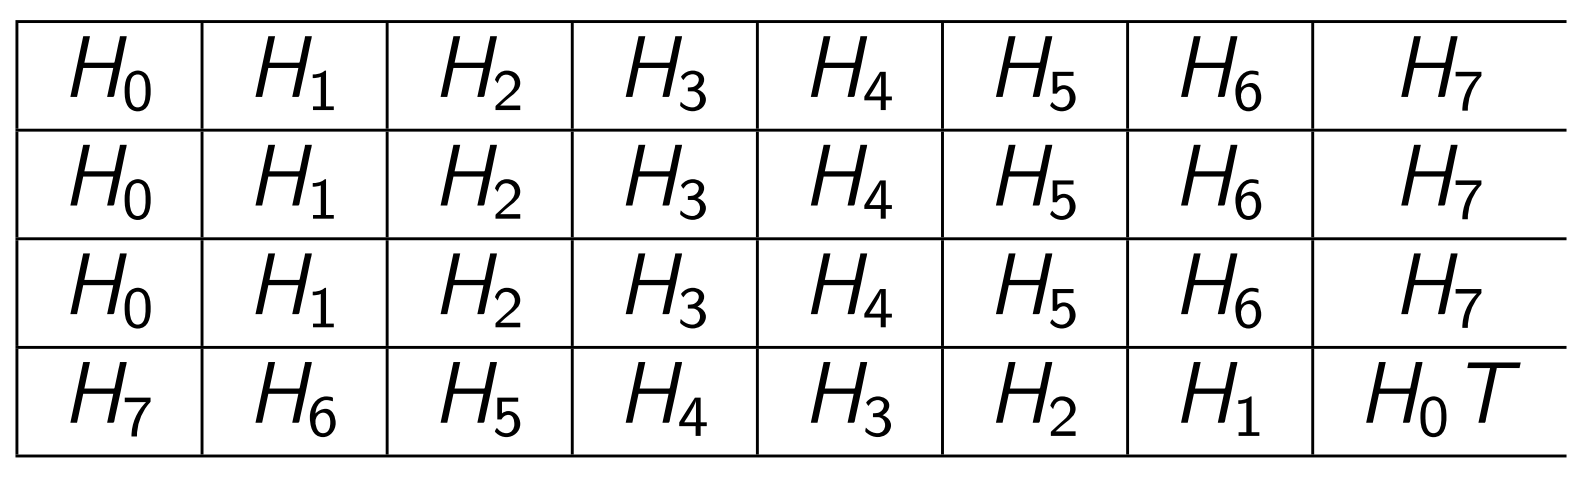
\includegraphics[width=\linewidth]{gost}
		\caption{Схематичная работа алгоритма ГОСТ}
	\end{figure}

	Описать трудоемкость, вероятность успеха, затраты по памяти и объём материала для методов Исобе и Динура-Данкельмана-Шамира.
	
	\subsection*{Метод Исобе}
	
	Для начала определим количество материала, необходимое для однозначного опредления ключа. Поскольку одной на паре $(P, C)$ открытого и шифрованного текста, где $P, C \in V_{64}$, можно отбраковать $2^{64}$ ключей, то потребуется $\ceil{\frac{256}{64}} = 4$ различные пары: $(P_1, C_1), (P_2, C_2), (P_3, C_3), (P_4, C_4)$. Будем дальше считать, что они нам даны.
	
	Теперь зафиксируем свойство алгоритма ГОСТ, которое поможет нам в построении эффективного алгоритма получения ключа. Пусть $(X, Y)$ -- пара входа-выхода на 4 итерациях алгоритма ГОСТ, 
	а $K_i, K_{i+1}, K_{i+2}, K_{i+3} \in V_{32}$ -- итерационные ключи этих 4 итераций.
	
	\begin{property}[Четырёх операций] \label{prop:4op}
		При известных $(X, Y)$ и при фиксации ключей $K_{i}, K_{i+1}$ (или $K_{i+2}, K_{i+3}$) конкретными значениями, два других ключа определяются однозначно.
	\end{property}
	
	Будем считать, что нам дана возможность по любому открытому тексту получить его зашифрованную версию, иными словами для любого открытого текста $P$ мы можем вычислить $E(P, K)$ даже не зная $K$ (это может быть заранее полученный корпус из пар открытый-закрытый тексты).
	
	Обозначим за $F_K^{[i, j]}(P)$ результат зашифрования на ключе $K$ алгоритмом ГОСТ, начиная с итерации с номером $i$, и заканчивая итерацией с номером $j$ $(1 \le i \le j \le 32)$ текста $P$.

	
	\begin{algorithm}[H]
		
		\caption{Метод Исобе}
		\label{alg:Isobe}
		\SetAlgoNoEnd 
		
		\KwData{Пары открытого и шифрованного текста $(P_1, C_1), (P_2, C_2), (P_3, C_3), (P_4, C_4)$}
		\KwResult{Ключ шифрования $K$}
	
	
		Принять $i=1$
		
		\While{ключ не найден или $i > 2^{32}$}{
			
			$i=i+1$
			
			Выберем случайно $P \in V_{64}$ -- открытый текст
			
			Посчитаем $C=E(P, K)$ 

			\ForEach{$(S, T) \in V_{128}$}{	
				
				\tcc{тут $S$ и $T$ - это внутренние состояния после 4 и 12 итераций соответсвенного}
				
				\ForEach{$(K_4, K_5) \in V_{64}$}{
					
					По свойству \ref{prop:4op} находим $(K_6, K_7) \in V_{64}$ по известным $T, C, K_4, K_5$
					
					Обозначаем $K'=(K_4, K_5, K_6, K_7)$
					
					Вычисляем $V=F_{K'}^{[5,8]}(S)$
					
					Заносим в память по адресу $V$ значение ключа $K'$
						
				}
				
				\ForEach{$(K_0, K_1) \in V_{64}$}{
					
					По свойству \ref{prop:4op} находим $(K_2, K_3) \in V_{64}$ по известным $P, S, K_0, K_1$
					
					Обозначаем $K''=(K_0, K_1, K_2, K_3)$
					
					Вычисляем $U={F^{-1}}_{K''}^{[9,12]}(T)$
					
					Извлекаем из памяти по адресу $U$ ключ $K'$
					
					Обозначаем $K=(K'', K') \in V_{256}$
					
					Доопробуем ключ $K$ на парах $(P_i, C_i), i \in \overline{1,4}$
					
					\If{доопробование успешно,}{
						Вернуть ключ $K$ и завершить алгоримт
					}
				}
			
			}			
		}
	\end{algorithm}	

	Алгоритм \ref{alg:Isobe} был сформулирован как вероятностный, чтобы продемонстрировать его основные характеристики. Детеременированная версия алгоритма (вероятность успеха которой равна 1) легко получается заменой случайного выбора на перебор всевозможных значений. 
	
	Возвращаясь к рассуждениям о получении шифртекста по открытому тексту, стоит заметить, что данная формулировка алогритма используется тот факт, что объём построенного заранее корпуса данных должен быть не менее $2^{32}$ пар открытый-закрытый тексты. Вероятность попадания в неподвижную точку преобразования $H T H^{-1}$ равна $2^{-32}$. Из-за этого при наличии корпуса размером $2^{32}$ мы в среднем попадём в 1 неподвижную точку и в среднем доопробуем ровно 1 ключ.
	
	Трудоёмоксть $Q$ этого алгоритма будем измерять в количествах использований свойства \ref{prop:4op} и вычислений 4 итераций алгоритма ГОСТ (поскольку в алгоритме Исобе одна операция идёт строго за другой, то можно выбрать любую на усмотрение). Необходимую для работы алгоритма память $M$ будем измерять в битах. Тогда имеем
	
	\[ Q = 2^{32} \cdot 2^{128} \cdot (2^{64} + 2^{64}) = 2^{225} \]
	
	\[ M = 2^{64} * 128 + \alpha = 2^{71} + \alpha,  \]
		
	где $\alpha$ - количество памяти, необходимое для хранения локальных переменных алгоритма.
	
	Вероятность успеха (наличия на доступном материале неподвижной точки) равна	
	\[ p=1-(1-\frac{1}{2^{32}})^{2^{32}} \approx 1 - e^{-1} \approx 0.63. \]
		
\end{document}
